%% Beispiel-Präsentation mit LaTeX Beamer im KIT-Design
%% entsprechend den Gestaltungsrichtlinien vom 1. August 2020
%%
%% Siehe https://sdqweb.ipd.kit.edu/wiki/Dokumentvorlagen

%% Beispiel-Präsentation
\documentclass[en]{sdqbeamer} 

\usepackage[svgnames]{xcolor}

%% Footnote without numbering
\newcommand\nonumberfootnote[1]{%
  \begingroup
  \renewcommand\thefootnote{}\footnote{#1}%
  \addtocounter{footnote}{-1}%
  \endgroup
}

%% Titelbild
\titleimage{banner_2020_kit}

%% Gruppenlogo
\grouplogo{} 

%% Gruppenname und Breite (Standard: 50 mm)
\groupname{Institute for Automation and Applied Informatics (IAI)}
\groupnamewidth{60mm}

% Beginn der Präsentation

\title[ABAC for Substations]{Certificateless Attribute-Based Server-Aided Cryptosystem\\for Substation Automation Systems (CASC-SAS)}
\subtitle{Master's Thesis Presentation} 
\author[Moritz Gstuer]{Moritz Gstuer}

\date[12.\,02.\,2025]{12. February 2025}

% Literatur
\usepackage[citestyle=authoryear,bibstyle=numeric,hyperref,maxcitenames=2,backend=biber]{biblatex}
\addbibresource{../bibliography/masterthesis.bib}
\bibhang1em

\begin{document}
 
%Titelseite
\KITtitleframe

%Inhaltsverzeichnis
%\begin{frame}{Agenda}
%\tableofcontents
%\end{frame}

\section{Motivation}
\begin{frame}{Motivation}
    \begin{columns}
        \column{.55\textwidth}
        \centering
        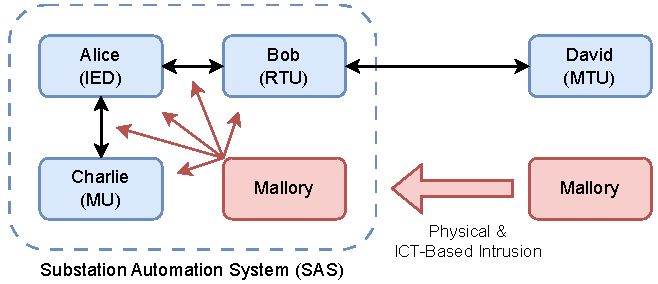
\includegraphics[width=1.0\textwidth]{./figures/sas_intrusion.drawio.pdf}
        \column{.45\textwidth}
        \begin{redblock}{Cyberattacks}
            \begin{itemize}
                \item \textbf{Availability-Focused:} Denial-of-Service\\$\rightarrow$ Malware, Flooding, \& Time-Delay
                \item \textbf{Integrity-Focused:} False Data Injection\\$\rightarrow$ Message Forgery, Modification, \& Replay
                \item \textbf{Authenticity-Focused:} Masquerading\\$\rightarrow$ Adaptive Chosen-Message, \& Collusion
            \end{itemize}
            % $\rightarrow$ Authentication, Authorization, Access Control, \& Encryption of Substation Communication
        \end{redblock}
    \end{columns}
    \nonumberfootnote{\color{SteelBlue} IED\dots Intelligent Electronic Device \color{black}| \color{SteelBlue} RTU\dots Remote Terminal Unit \color{black}| \color{SteelBlue} MTU\dots Master Terminal Unit \color{black}| \color{SteelBlue} MU\dots Merging Unit}
    \nonumberfootnote{ICT\dots Information and Communications Technology}
\end{frame}
\begin{frame}{Substation Communication}
    \begin{blueblock}{Requirements}
        \begin{columns}[T, onlytextwidth]
            \column{.50\textwidth}
            \begin{itemize}
                \setlength{\itemindent}{-1em}
                \item Integrity
                \item Authenticity
                \item Non-Repudiation
            \end{itemize}
            $\rightarrow$ \textbf{Authentication}
            \column{.50\textwidth}
            \begin{itemize}
                \setlength{\itemindent}{-1em}
                \item Prevention of Unauthorized Access
                \item Least Privilege Principle
                \item Separation of Duties
            \end{itemize}
            $\rightarrow$ \textbf{Authorization \& Access Control}
        \end{columns}
    \end{blueblock}
    \begin{grayblock}{Constraints: IEC 61850 Message Types \& Performance Classes \parencite*{IEC61850P5,IEC61850P8}}
        Client-Server (Unicast) \& Publisher-Subscriber (Broadcast/Multicast) \\$\rightarrow$ Resource \& Time Constraints!
        \\Examples: GOOSE (Type 1A, 3 ms), SV (Type 4, 3 ms), MMS (Type 2/3/5, 100-10000 ms)
    \end{grayblock}
    \nonumberfootnote{GOOSE\dots Generic Object Oriented Substation Event | SV\dots Sampled Values | MMS\dots Manufacturing Message Specification}
\end{frame}
\begin{frame}{Research Questions}
    \begin{greenblock}{\textbf{RQ 1:} Authorization \& Access Control in Substation Automation System}
        How can \textbf{expressive} and \textbf{flexible} yet computationally expensive \textbf{access control} be employed in a SAS?
    \end{greenblock}

    \begin{greenblock}{\textbf{RQ 2:} Public-Key Cryptography in Substation Automation System}
        How can a \textbf{secure} and \textbf{lightweight} \textbf{public-key approach} be designed, implemented, \& employed in a SAS?
    \end{greenblock}

    \begin{greenblock}{\textbf{RQ 3:} Security Architecture for Time-Critical Communication}
        How can \textbf{authentication}, \textbf{authorization}, and \textbf{access control} be integrated into a malleable, scalable, and lightweight \textbf{cryptosystem for time-critical SAS communication}?
    \end{greenblock}
\end{frame}

\section{Fundamentals}
\begin{frame}{Attribute-Based Access Control (ABAC)}
    \begin{greenblock}{Definition \parencite{JTF2020}}
        Access control model enabling access decisions based on attributes associated with \textbf{subjects}, \textbf{objects}, \textbf{actions}, and the \textbf{environment} of a system.
    \end{greenblock}
    \begin{blueblock}{Discussion \parencite{Hu2014}}
        \begin{itemize}
            \item Multifactor Policy Expression $\rightarrow$ Fine-Grained \& Flexible Access Control (cf. RBAC/IBAC)
            \item Dynamic Policy Evaluation $\rightarrow$ Dynamic Authorization \& Real-Time Attributes
        \end{itemize}
    \end{blueblock}
\end{frame}
\begin{frame}{Public-Key Cryptography in SAS}
    \begin{blueblock}{Key Distribution \& Identity Verification}
        Unsecure Network \& Untrusted Network Participants
        \\$\rightarrow$ Asymmetric: Lightweight \& Secure Key Distribution
    \end{blueblock}
    \begin{blueblock}{Computational Complexity \parencite{Elbez2019,Ishchenko2018}}
        Example: 1024-Bit RSA Digital Signature vs. 128-Bit HMAC/GMAC
        \\$\rightarrow$ 10 ms vs. 50 µs on RPi2 (1 GHz quad-core)
        \\$\rightarrow$ 0.3 ms vs. 4 µs on Xeon X3440 (2.53 GHz quad-core) 
    \end{blueblock}
\end{frame}

\section{Problem Statement}
\begin{frame}{Norms \& Standards}
    \begin{blueblock}{IEC 62351: Part 6 \& Part 8 \parencite*{IEC62351P6,IEC62351P8}}
        Standard for Cybersecurity: Energy-Related Systems \& Communication Networks
        \\$\rightarrow$ \textbf{Authenticity \& Integrity:} Mandatory Symmetric Authentication
        \\$\rightarrow$ \textbf{Confidentiality:} Optional (Non-Recommended) Symmetric Encryption
        \\$\rightarrow$ \textbf{Access Control:} Role-Based Access Control (RBAC) (Access-Token-Driven, 7 Mandatory Roles)
    \end{blueblock}
\end{frame}
\begin{frame}{Related Work}
    \begin{blueblock}{Secure Communication in Substations}
        \begin{itemize}
            \item Bump-in-the-Wire Security Filter for \textbf{GOOSE/SV MAC Tagging} \& Verification \parencite{Ishchenko2018}
            \item \textbf{Domain-Based Collaborative} Cyberattack Mitigation Approach \parencite{Hong2019}
            \item Fixed-Latency Hardware Architecture for \textbf{GOOSE/SV Encryption} \& Authentication \parencite{Rodriguez2021}
        \end{itemize}
    \end{blueblock}

    \begin{blueblock}{Access Control in Substations}
        \begin{itemize}
            \item XACML-Based \textbf{RBAC} Approach for IEC 61850 \& IEC 62351 compliant SAS \parencite{Lee2015}
            \item Distributed \textbf{RBAC} for Subscription-Based Remote Network Services \parencite{Ma2006} % Constraint-Enabled 
            \item Rule-Based \textbf{RBAC} Policy Enforcement Architecture \parencite{Alcaraz2016} % for Smart Grid Systems
            \item Firewall for \textbf{ABAC} in Smart Grids \parencite{Ruland2018}
            \item \textbf{ABAC} for Real-Time Availability in Highly Dynamic Systems \parencite{Burmester2013}
        \end{itemize}
    \end{blueblock}
\end{frame}
\begin{frame}{Research Gap \& Contributions}
    \begin{redblock}{Limitations of Related Work}
        Missing consolidation of secure communication \& access control in substations
        \\$\rightarrow$ \textbf{Consolidation of Competencies:} Increase security \& performance, \& facilitate deployment
    \end{redblock}
    \begin{greenblock}{Contributions}
        \begin{itemize}
            \item Requirements \& constraints of the \textbf{field of application}
            \item \textbf{Authorization} \& \textbf{access control} approach based on ABAC $\rightarrow$ \textbf{RQ 1}
            \item Algorithm-agnostic \textbf{authentication} framework \& attribute-based signature scheme $\rightarrow$ \textbf{RQ 2}
            \item \textbf{Security architecture} integrating authentication, authorization, \& access control $\rightarrow$ \textbf{RQ 3}
            \item Security, performance, \& compatibility \textbf{evaluation} of the approach
        \end{itemize}
    \end{greenblock}
\end{frame}

\section{Approach}
\begin{frame}{Approach: Overview}
    \begin{columns}[T, onlytextwidth]
        \column{.60\textwidth}
        \begin{greenblock}{Approach}
            \textbf{C}ertificateless \textbf{A}ttribute-Based \textbf{S}erver-Aided \textbf{C}ryptosystem for \textbf{S}ubstation \textbf{A}utomation \textbf{S}ystems (CASC-SAS)\\
            \vspace{1em}
            \textbf{Objective:} Fine-grained \& flexible access control relying on dynamic authorization \& authentication
            \vspace{1em}
            \\\textbf{Central Concepts:}
            \begin{itemize}
                \item Authentication $\rightarrow$ CASA
                \item Authorization \& Access Control $\rightarrow$ SABAAC
            \end{itemize}
        \end{greenblock}
        \column{.40\textwidth}
        \centering
        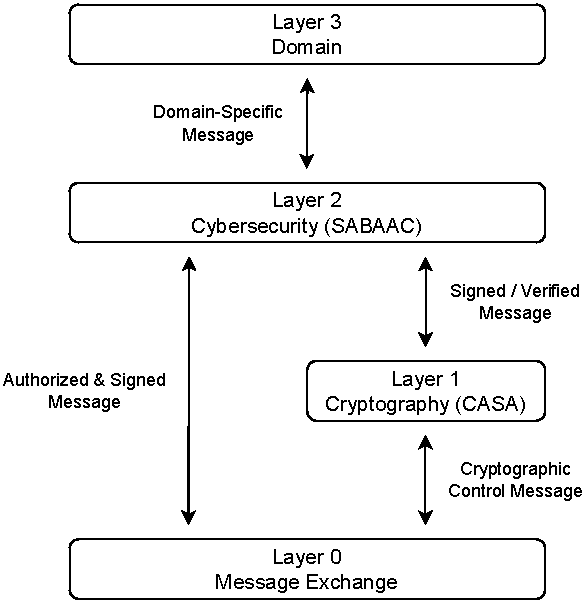
\includegraphics[width=0.80\textwidth]{./figures/layers_request_example_shortened.drawio.pdf}
    \end{columns}
    \nonumberfootnote{CASA\dots Certificateless Attribute-Based Server-Aided Authentication}
    \nonumberfootnote{SABAAC\dots Server-Aided Attribute-Based Authorization \& Access Control}
\end{frame}
\begin{frame}{CASA: Authentication}
    \begin{greenblock}{\textbf{C}ertificateless \textbf{A}ttribute-Based \textbf{S}erver-Aided \textbf{A}uthentication (CASA)}
        Lightweight \& scalable algorithm-agnostic data frame authentication approach
        \\\textbf{Additionally:} $S_{CASA}$ $\rightarrow$ Certificateless attribute-based server-aided signature scheme
    \end{greenblock}
    \begin{blueblock}{Protocol: Algorithm-Agnostic PKC Exchange}
        \textbf{Tasks:} Registration, revocation, query, \& computation
        \\\textbf{Central Component:} CASA Administration and Processing Platform (CAPP)
    \end{blueblock}
    \nonumberfootnote{PKC\dots Public Key Cryptography}
\end{frame}
\begin{frame}{SABAAC: Authorization \& Access Control}
    \begin{greenblock}{\textbf{S}erver-Aided \textbf{A}ttribute-\textbf{B}ased \textbf{A}uthorization \& \textbf{A}ccess \textbf{C}ontrol (SABAAC)}
        Delegation of access policy evaluation to semi-trusted server (PDP)
        \\$\rightarrow$ Enforcement of access control decisions via bump-in-the-wire device (PEP)
    \end{greenblock}
    \begin{blueblock}{Protocol: Delegated Attribute-Based Authorization}
        \textbf{Task:} Creation, modification, storage, and distribution of access control policies
        \\\textbf{Central Components:} PAP \& PDP
    \end{blueblock}
    \begin{blueblock}{Protocol: Delegated Attribute-Based Access Control}
        \textbf{Task:} Request, exchange, \& enforcement of access control decisions
        \\\textbf{Central Components:} PDP \& PEP
    \end{blueblock}
    \nonumberfootnote{PAP\dots Policy Administration Point | PDP\dots Policy Decision Point | PEP\dots Policy Enforcement Point}
\end{frame}
\begin{frame}{Delegated Access Control: Session Initialization}
    \centering
    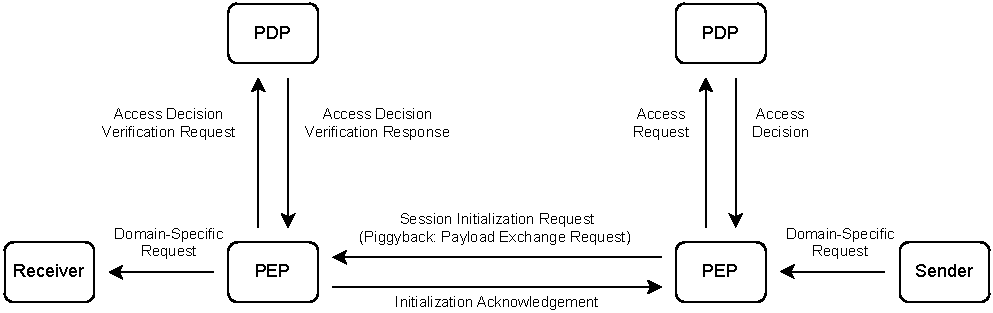
\includegraphics[width=1.0\textwidth]{./figures/SABAAC_protocols_accesscontrol_initialization_shortened.drawio.pdf}
    \nonumberfootnote{\color{IndianRed} PDP\dots Policy Decision Point}
    \nonumberfootnote{\color{IndianRed} PEP\dots Policy Enforcement Point}
\end{frame}
\begin{frame}{Delegated Access Control: Payload Exchange}
    \centering
    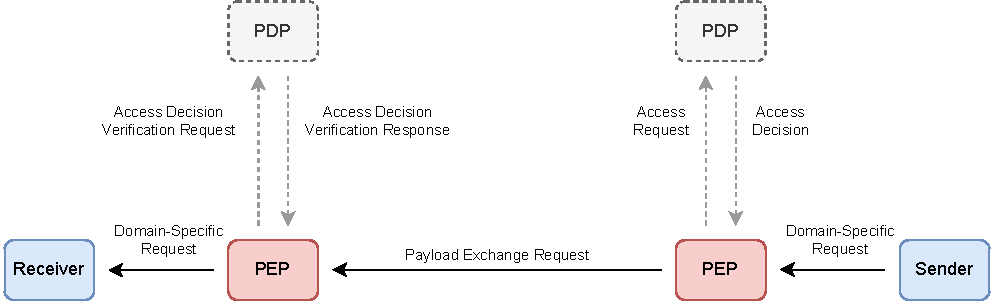
\includegraphics[width=1.0\textwidth]{./figures/SABAAC_protocols_accesscontrol_payloadexchange_with_pdp.drawio.pdf}
    \nonumberfootnote{\color{Grey} PDP\dots Policy Decision Point}
    \nonumberfootnote{\color{IndianRed} PEP\dots Policy Enforcement Point}
\end{frame}
\begin{frame}{CASC-SAS: Component-Oriented Architecture}
    \begin{columns}
        \column{.65\textwidth}
        \centering
        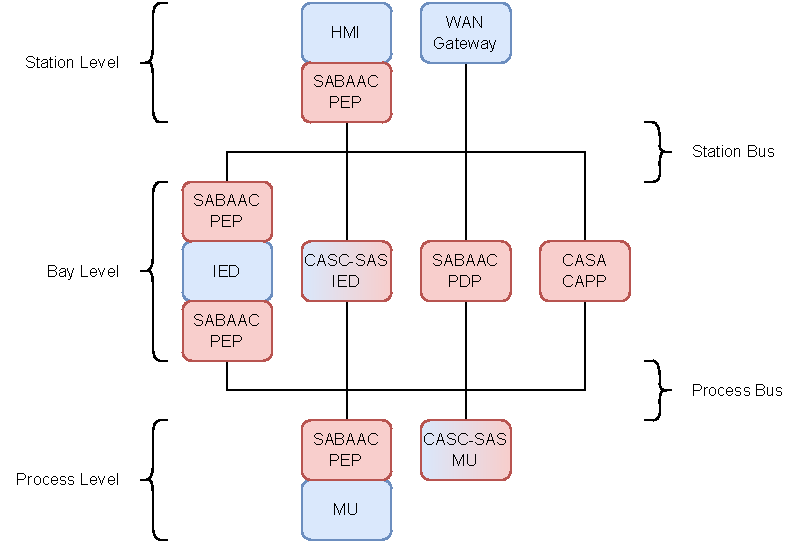
\includegraphics[height=0.75\textheight]{./figures/casc_architecture_color_shortened.drawio.pdf}
        \column{.35\textwidth}
        \footnotesize
        \begin{center}
            \begin{tabular}{r l}
                \color{IndianRed} CAPP & \color{IndianRed} CASA Administration \\
                     & \color{IndianRed} \& Processing Platform \\
                \color{IndianRed} PDP & \color{IndianRed} Policy Decision Point \\
                \color{IndianRed} PEP & \color{IndianRed} Policy Enforcement Point \vspace{1em}\\
                \color{SteelBlue} HMI & \color{SteelBlue} Human-Machine Interface \\
                \color{SteelBlue} IED & \color{SteelBlue} Intelligent Electronic Device \\
                \color{SteelBlue} MU & \color{SteelBlue} Merging Unit \\
                \color{SteelBlue} WAN & \color{SteelBlue} Wide Area Network
            \end{tabular}
        \end{center}
    \end{columns}
\end{frame}

\section{Evaluation}
\begin{frame}{Evaluation: Overview}
    \begin{greenblock}{Goal of Approach}
        Protect substations against domain-typical adversaries \& attacks
        \\\textbf{Communication:} Time-Constrained \& Traffic-Intensive
        \\\textbf{Deployment:} Construction \& Retrofitting
    \end{greenblock}
    \begin{blueblock}{Evaluation}
        Theoretically \& experimentally performed evaluation
        \begin{itemize}
            \item Security Analysis
            \item Performance Analysis
            \item Compatibility Analysis
        \end{itemize}
    \end{blueblock}
\end{frame}
\begin{frame}{Security Analysis}
    \begin{greenblock}{Central Question}
        To what extent does CASC-SAS provide security against typical SAS adversaries and attacks?
        \\\textbf{Metrics:} Satisfied requirements, assumed adversary, mitigated attacks, \& change of substation attack surface
    \end{greenblock}
    \begin{blueblock}{Theorems}
        Demonstration of the reduced likelihood and impact of six attacks:
        \vspace{1em}
        \begin{columns}[T, onlytextwidth]
            \column{.40\textwidth}
            \textbf{Integrity-Focused Attacks}
            \begin{itemize}
                \item Message Creation
                \item Message Modification
                \item Message Replay
                \item Message Delay
            \end{itemize}
            \column{.60\textwidth}
            \textbf{Authenticity-Focused Attacks}
            \begin{itemize}
                \item Collusion
                \item Existential Unforgeability under Chosen-Message Attacks
            \end{itemize}
        \end{columns}
    \end{blueblock}
\end{frame}
\begin{frame}{Performance Analysis}
    \centering
    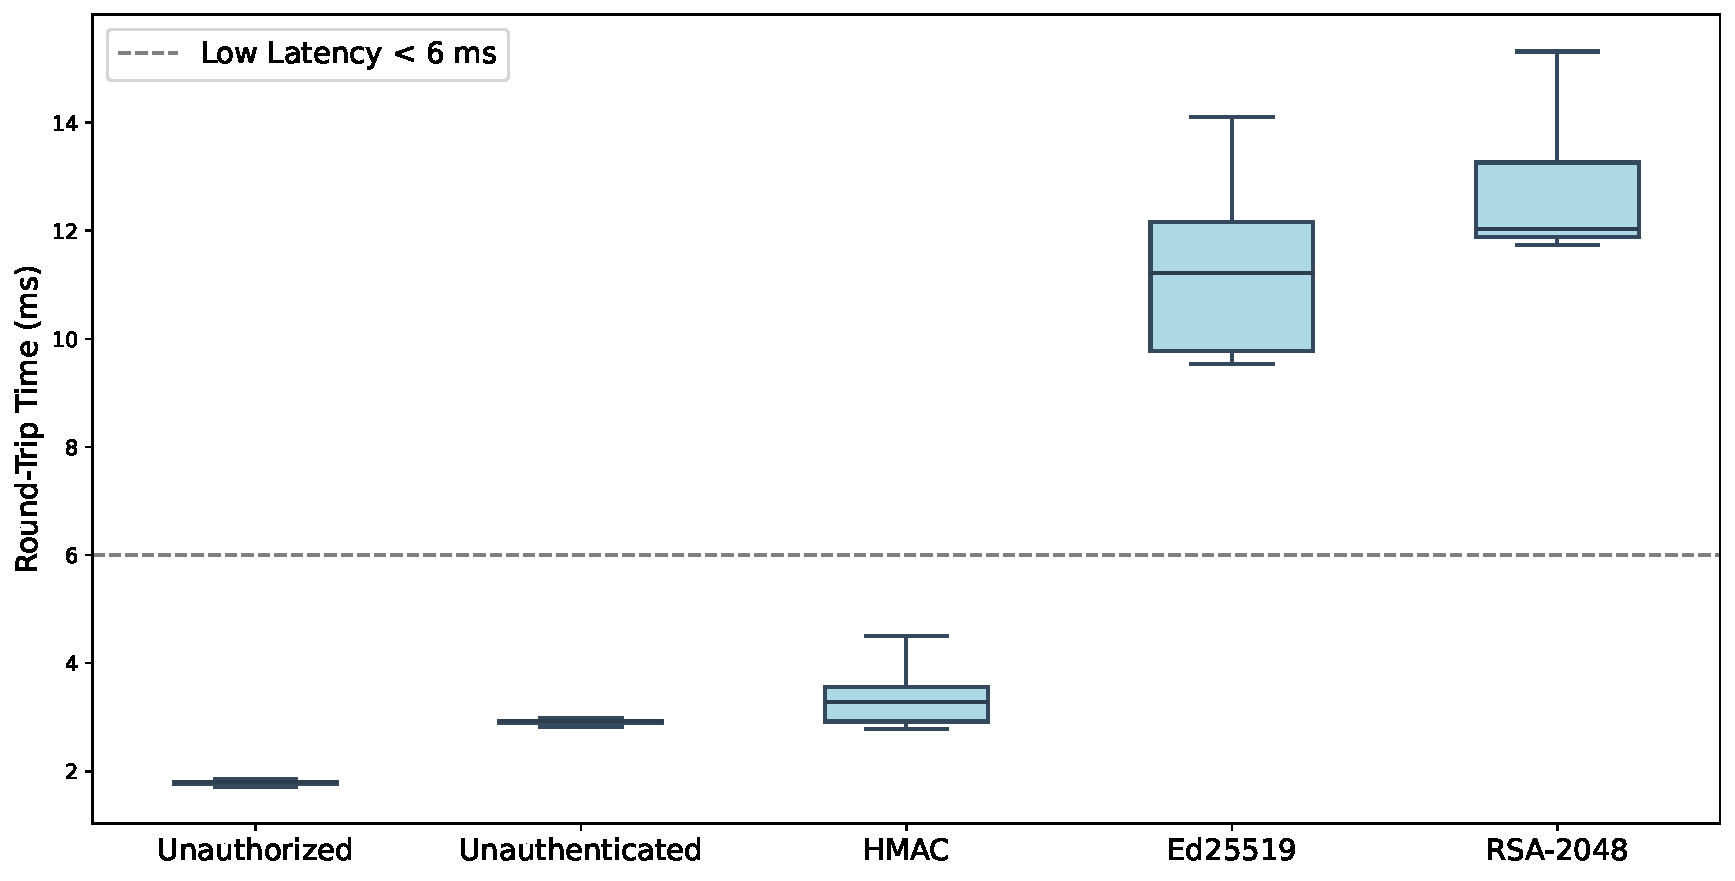
\includegraphics[height=0.75\textheight]{./figures/boxplot_without_casa.pdf}
\end{frame}
\begin{frame}{Performance Analysis}
    \centering
    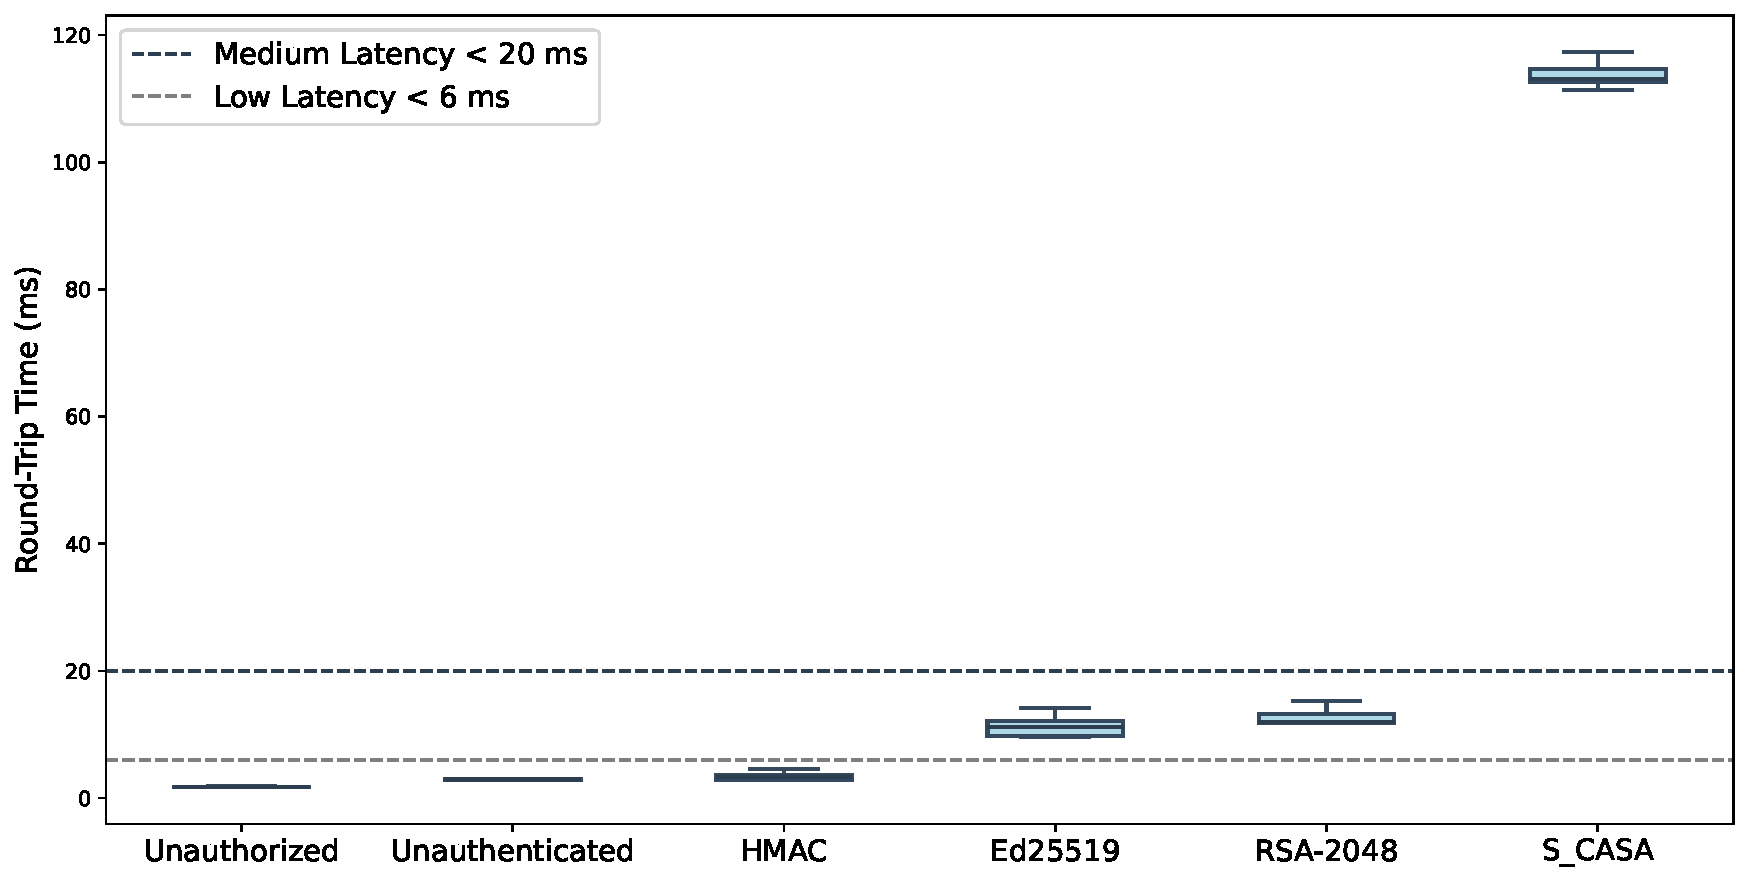
\includegraphics[height=0.75\textheight]{./figures/boxplot_with_casa.pdf}
\end{frame}
\begin{frame}{Performance Analysis: $S_{CASA}$}
    \begin{redblock}{Message Exchange Round-Trip Time}
        \begin{center}
            \begin{tabular*}{0.8\linewidth}{@{\extracolsep{\fill}} c c c c }
                \textbf{Minimum} & \textbf{Average} & \textbf{Maximum} & \textbf{Deviation}\\
                $\approx$ 111 ms & $\approx$ 120 ms & $\approx$ 510 ms & $\approx$ 29 ms
            \end{tabular*}
        \end{center}
    \end{redblock}
    \begin{greenblock}{Speedup Solutions}
        \begin{itemize}
            \item Optimization of implementation
            \item Hardware acceleration
        \end{itemize}
    \end{greenblock}
    \begin{blueblock}{Cryptography-Driven Authentication, Authorization, \& Access Control}
        Authentication, authorization, \& access control integrated into a single attribute-based PKC scheme
        \\$\rightarrow$ \textbf{Advantage:} Privacy \& Anonymity
    \end{blueblock}
\end{frame}
\begin{frame}{Compatibility Analysis}
    \centering
    \includegraphics<1>[height=0.70\textheight]{./figures/lab_evaluation_steps_simplified_step0.drawio.pdf}%
    \includegraphics<2>[height=0.70\textheight]{./figures/lab_evaluation_steps_simplified_step1.drawio.pdf}%
    \includegraphics<3>[height=0.70\textheight]{./figures/lab_evaluation_steps_simplified_step2.drawio.pdf}%
    \includegraphics<4>[height=0.70\textheight]{./figures/lab_evaluation_steps_simplified_step3.drawio.pdf}%
    \includegraphics<5>[height=0.70\textheight]{./figures/lab_evaluation_steps_simplified.drawio.pdf}%
    \nonumberfootnote{\color{IndianRed} PDP\dots Policy Decision Point \color{black}| \color{IndianRed} PEP\dots Policy Enforcement Point}
\end{frame}

\section{Future Work}
% \begin{frame}{Future Work I}
%     \begin{blueblock}{Cryptography-Driven Authentication, Authorization, \& Access Control}
%         Authentication, authorization, \& access control integrated into a single attribute-based PKC scheme
%         \\$\rightarrow$ \textbf{Advantage:} Privacy \& Anonymity
%     \end{blueblock}
%     \begin{blueblock}{Encryption \& Decryption}
%         Encryption \& decryption in conjunction with signing \& verification operations
%         \\$\rightarrow$ \textbf{Advantage:} Confidentiality
%     \end{blueblock}
%     \begin{blueblock}{Hardware Acceleration}
%         Evaluation of hardware-based cryptography acceleration in a SAS
%         \\$\rightarrow$ \textbf{Advantage:} Decreased computation time \& increased message throughput
%         \\$\rightarrow$ \textbf{Risk:} Algorithm compatibility, costs per acceleration unit, \& computation time consistency
%     \end{blueblock}
% \end{frame}
\begin{frame}{Future Work}
    \begin{blueblock}{AI for Policy Management}
        Integration of CASC-SAS with AI-based intrusion detection for security policy creation \& modification
        \\$\rightarrow$ \textbf{Advantage:} Mitigation of a wider range of cyberattacks in a timelier manner
    \end{blueblock}
    \begin{blueblock}{SDN-Based Realization}
        Aggregation of PEPs by deploying a virtual PEP for each port of a Software-Defined Networking (SDN) switch
        \\$\rightarrow$ \textbf{Advantage:} Reduced costs of deployment \& reduced architectural complexity
    \end{blueblock}
    \begin{blueblock}{Extended Demonstration of Applicability}
        Employment in time-critical systems with similar requirements \& constraints
        \\$\rightarrow$ \textbf{Examples:} Industry 4.0, robotics, avionics, \& medical systems
    \end{blueblock}
\end{frame}

\section{Conclusion}
\begin{frame}{Conclusion}
    \begin{redblock}{Problem}
        Expressive \& flexible access control, \& malleable PKC: Applicable to the SAS domain?
        \\$\rightarrow$ Constrained resources \& communication time
    \end{redblock}
    \begin{blueblock}{Contribution}
        CASC-SAS security architecture \& framework\dots
        \\\dots employs mandatory authentication, authorization, \& access control
        \\\dots for time-critical SAS communication
        \\\dots in time-variable SAS environment.
    \end{blueblock}
    \vspace{0.5em}
    \centering
    \huge
    Thank you!
\end{frame}

\appendix
\beginbackup
\begin{frame}{~}
    \centering
    \Huge
    Appendix
\end{frame}
\section{System Model}
\begin{frame}{Adversarial Attacks}
    \begin{columns}
        \column{.38\textwidth}
        \centering
        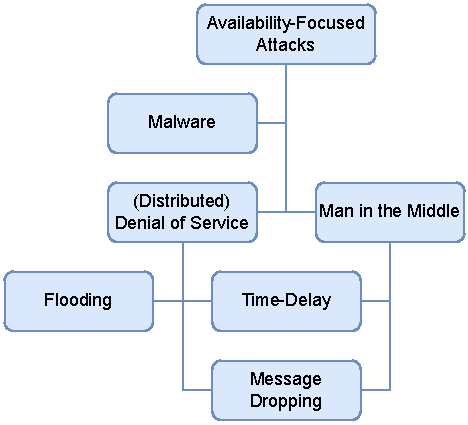
\includegraphics[width=\linewidth]{figures/attacks_availability.drawio.pdf}
        \column{.295\textwidth}
        \centering
        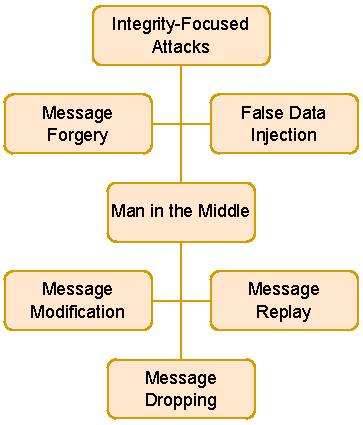
\includegraphics[width=\linewidth]{figures/attacks_integrity.drawio.pdf}
        \column{.30\textwidth}
        \centering
        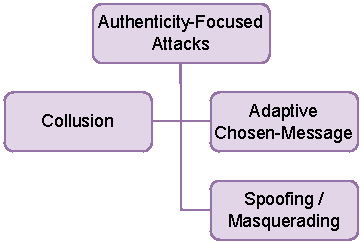
\includegraphics[width=\linewidth]{figures/attacks_authenticity.drawio.pdf}
    \end{columns}
\end{frame}
\begin{frame}{Substation Automation System (SAS)}
    \centering
    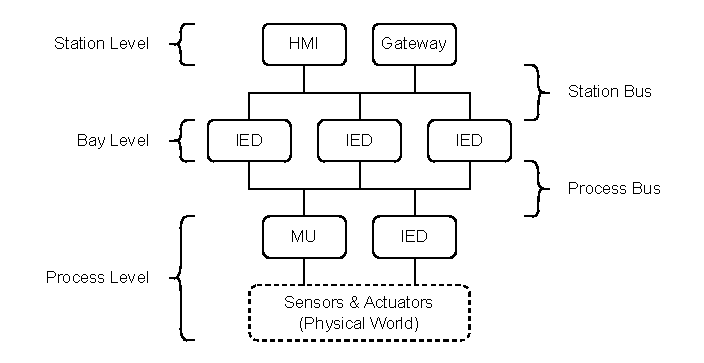
\includegraphics[width=0.7\textwidth]{./figures/substation_architecture.drawio.pdf}
    \nonumberfootnote{IED\dots Intelligent Electronic Device | MU\dots Merging Unit | HMI\dots Human-Machine Interface}
\end{frame}

\section{Fundamentals}
\begin{frame}{Authentication, Authorization, \& Access Control}
    \centering
	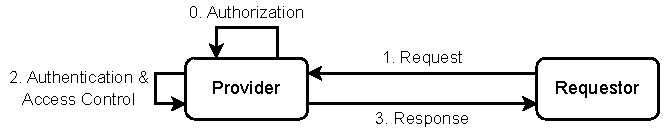
\includegraphics[width=0.9\textwidth]{./figures/access_control_request_traditional.drawio.pdf}
    \begin{redblock}{Problem}
        Too many provider responsibilities
        \\$\rightarrow$ Policy Management/Decisions/Enforcement, Request Verification, \& Response Creation
    \end{redblock}
\end{frame}

\section{Approach}
\begin{frame}{CASC-SAS Architecture: Function-Oriented}
    \centering
    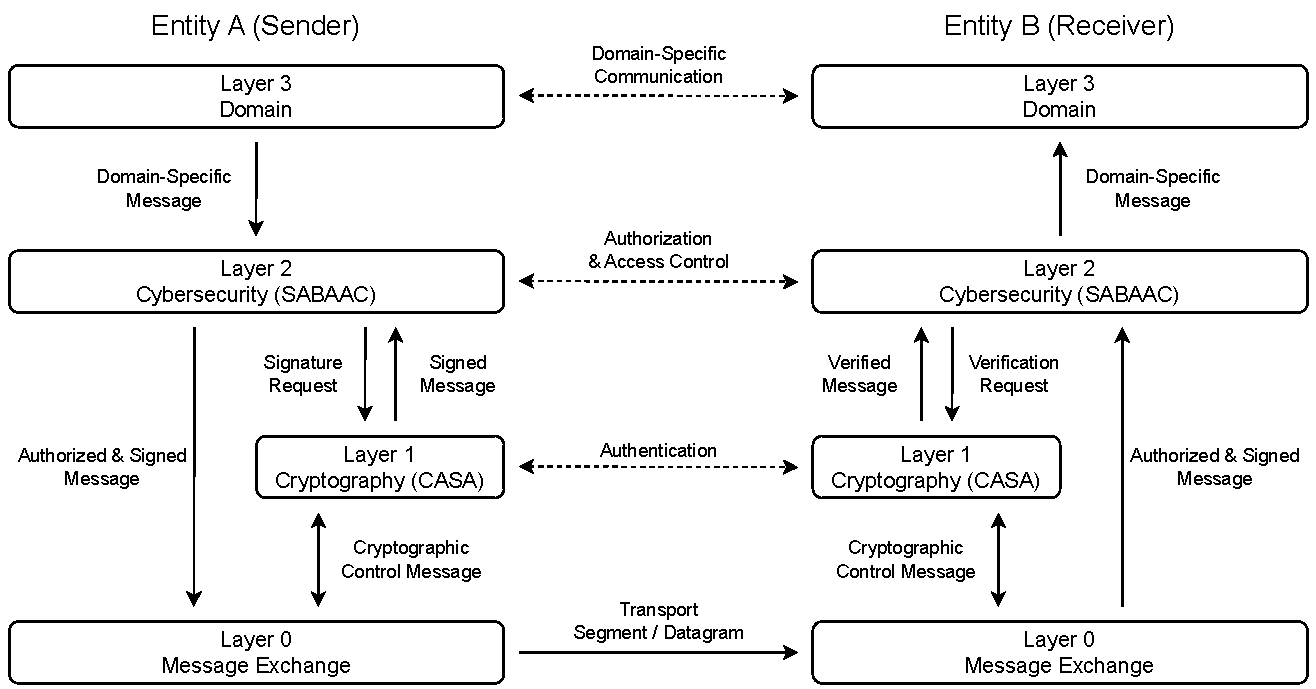
\includegraphics[height=0.75\textheight]{./figures/layers_request_example.drawio.pdf}
\end{frame}
\begin{frame}{CASC-SAS Architecture: Component-Oriented}
    \begin{columns}
        \column{.65\textwidth}
        \centering
        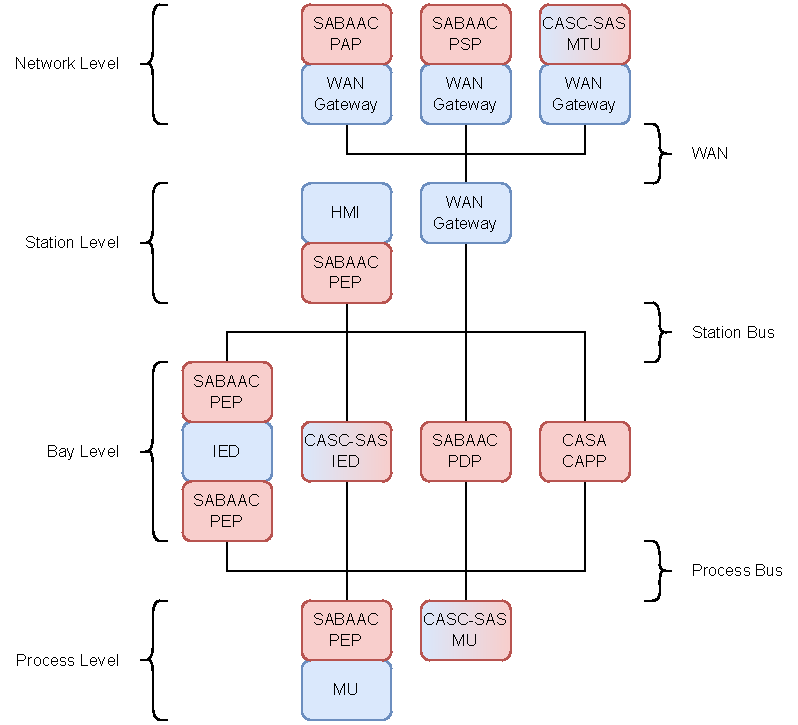
\includegraphics[height=0.75\textheight]{./figures/casc_architecture_color.drawio.pdf}
        \column{.35\textwidth}
        \footnotesize
        \begin{center}
            \begin{tabular}{r l}
                \color{IndianRed} CAPP & \color{IndianRed} CASA Administration \\
                     & \color{IndianRed} \& Processing Platform \\
                \color{IndianRed} PAP & \color{IndianRed} Policy Administration Point\\
                \color{IndianRed} PDP & \color{IndianRed} Policy Decision Point \\
                \color{IndianRed} PEP & \color{IndianRed} Policy Enforcement Point\\
                \color{IndianRed} PSP & \color{IndianRed} Policy Storage Point \vspace{1em}\\
                %
                \color{SteelBlue} HMI & \color{SteelBlue} Human-Machine Interface \\
                \color{SteelBlue} IED & \color{SteelBlue} Intelligent Electronic Device \\
                \color{SteelBlue} MTU & \color{SteelBlue} Master Terminal Unit\\
                \color{SteelBlue} MU & \color{SteelBlue} Merging Unit \\
                \color{SteelBlue} WAN & \color{SteelBlue} Wide Area Network
            \end{tabular}
        \end{center}
    \end{columns}
\end{frame}
\begin{frame}{SABAAC: Static Authorization}
    \centering
    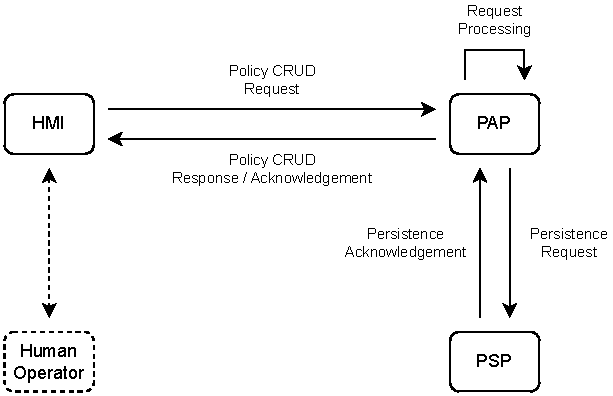
\includegraphics[height=0.75\textheight]{./figures/SABAAC_protocols_authorization_static.drawio.pdf}
\end{frame}
\begin{frame}{SABAAC: Policy Exchange Incremental}
    \centering
    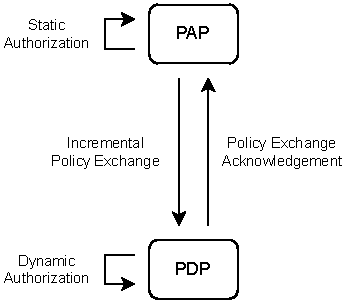
\includegraphics[height=0.75\textheight]{figures/SABAAC_protocols_authorization_dynamic_policyexchange_incremental.drawio.pdf}
\end{frame}
\begin{frame}{SABAAC: Policy Exchange Complete}
    \centering
    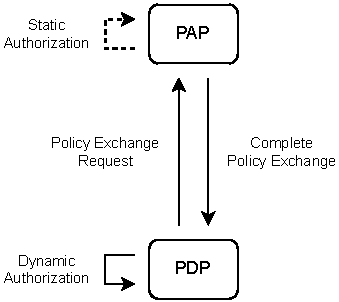
\includegraphics[height=0.75\textheight]{figures/SABAAC_protocols_authorization_dynamic_policyexchange_complete.drawio.pdf}
\end{frame}
\begin{frame}{SABAAC: Dynamic Authorization}
    \centering
    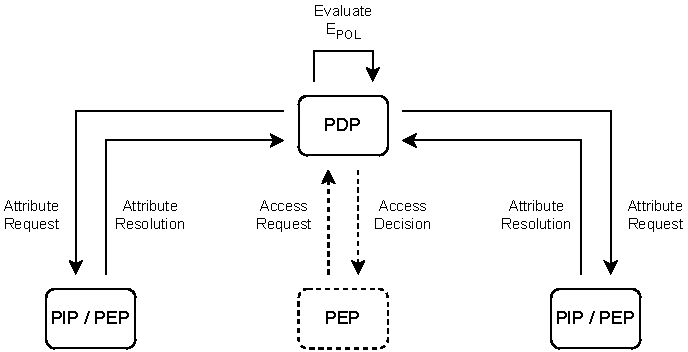
\includegraphics[height=0.75\textheight]{figures/SABAAC_protocols_authorization_dynamic.drawio.pdf}
\end{frame}
\begin{frame}{SABAAC: Session Initialization Piggybacking}
    \centering
    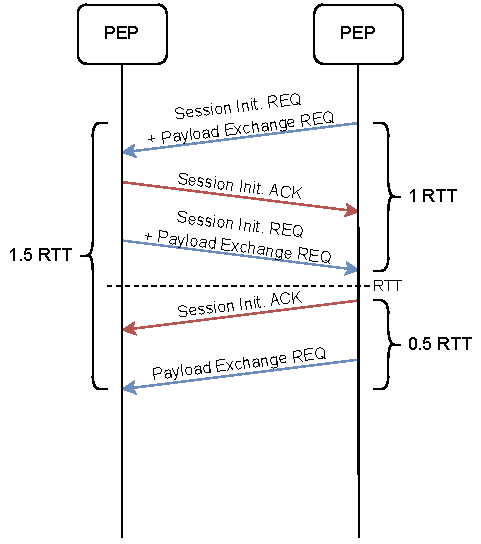
\includegraphics[height=0.75\textheight]{figures/SABAAC_protocols_accesscontrol_initialization_rtt_piggyback.drawio.pdf}
\end{frame}

\section{Evaluation}
\begin{frame}{Performance Evaluation: Sequence of Events}
    \centering
    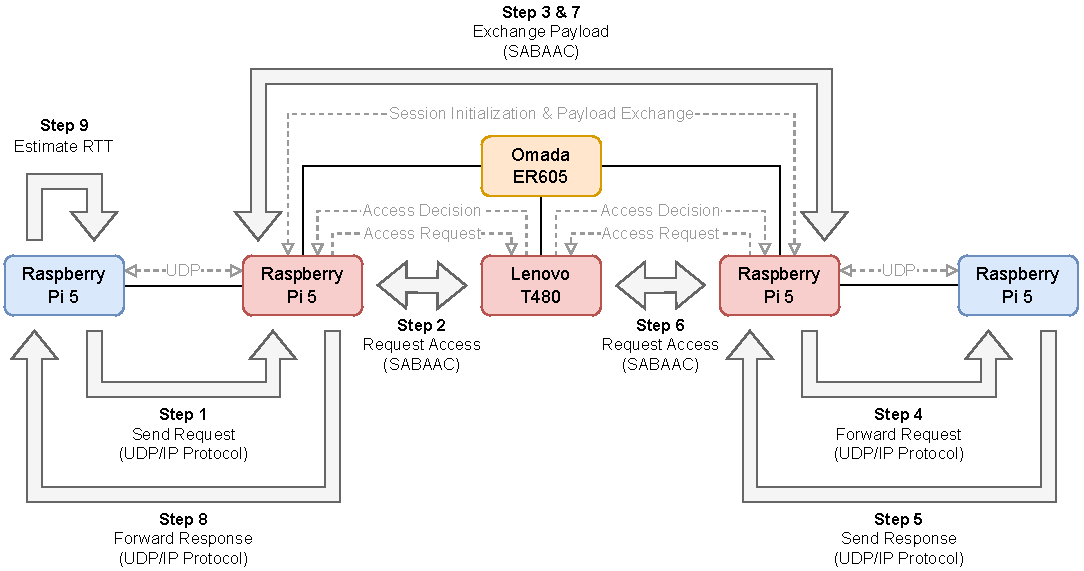
\includegraphics[height=0.75\textheight]{figures/performance_evaluation_steps.drawio.pdf}
\end{frame}

\section{Related Work}
\begin{frame}{Related Work: ABAC}
    \begin{blueblock}{Attribute-Based Access Control (ABAC)}
        \begin{itemize}
            \item T-ABAC: An attribute-based access control model for real-time availability in highly dynamic systems \parencite{Burmester2013}
            \item Firewall for Attribute-Based Access Control in Smart Grids \parencite{Ruland2018}
            \item An Attribute-Based Access Control for IoT Using Blockchain and Smart Contracts \parencite{Zaidi2021}
            \item A user-friendly attribute-based data access control scheme for smart grids \parencite{Mu2023}
            \item Accountable multi-authority attribute-based data access control in smart grids \parencite{Zhang2023}
            \item Secure Identities for Renewable Energy Sources Through Self-Sovereign Identity and Attribute-Based Access Control \parencite{Volkmann2024}
        \end{itemize}
    \end{blueblock}
    % Message Authentication, Asym. Performance Evaluation, BitW- \& HW-Solutions, Access Control
\end{frame}

\section{Paper}
\begin{frame}{Paper: ABS-SAS}
    \begin{greenblock}{Concept}
        Attribute-based signature (ABS) scheme for substation automation systems (SAS)
        \\$\rightarrow$ \textbf{Authentication \& authorization} via cryptographic scheme
    \end{greenblock}
    \begin{blueblock}{Work Plan}
        \textbf{Currently:} \textbf{Implementation} in C++, \& \textbf{evaluation} of the scheme with regard to security \& performance aspects\\
        \textbf{Soon:} \textbf{Discussion} of evaluation findings, \textbf{finalization} of paper, \& \textbf{proofreading}
    \end{blueblock}
    \begin{grayblock}{Submission (Planned)}
        \textbf{Workshop} @ 23rd International Conference on Applied Cryptography and Network Security (\textbf{ACNS}) in Munich
    \end{grayblock}
\end{frame}

\begin{frame}[allowframebreaks]{References}
\printbibliography
\end{frame}

\backupend

\end{document}